\chapter{Testdokumentation}\label{ch:testdokumentation}


\section{Normalfälle}\label{test:sec:normalfaelle}
\begin{center}
    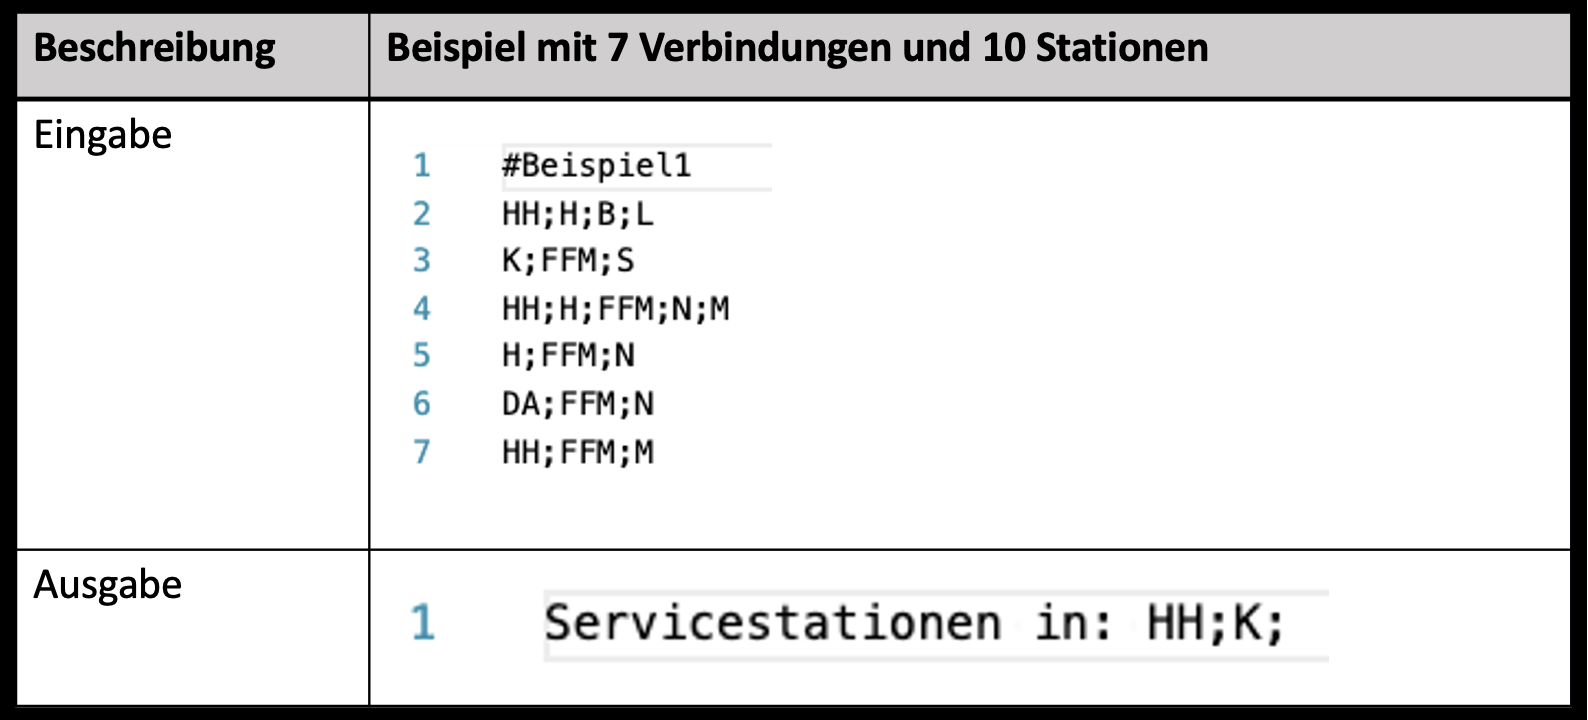
\includegraphics[width=\linewidth]{images/Tests/IHK-Beispiele/Beispiel1.png}
    \label{test:subsecpar:beispiel1}
\end{center}

\begin{center}
    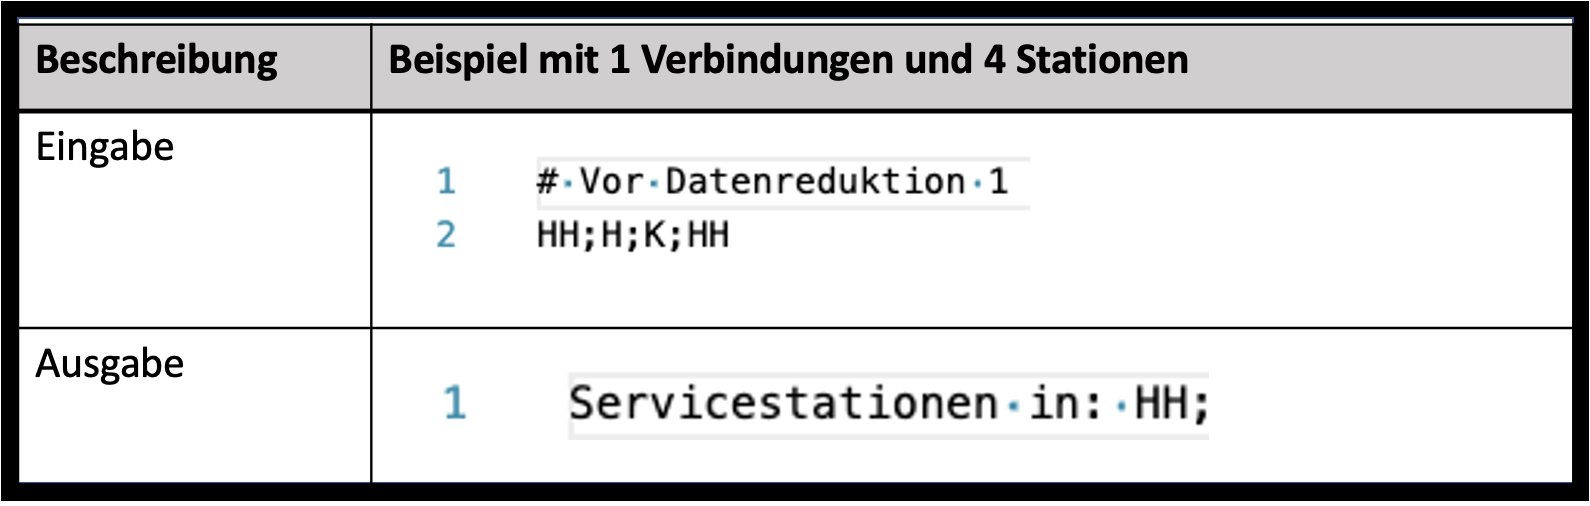
\includegraphics[width=\linewidth]{images/Tests/IHK-Beispiele/Datenreduktion1.png}
    \label{test:subsecpar:beispiel1}
\end{center}

\section{Fehlerfälle}\label{test:sec:fehlerfaelle}
Die folgenden Test decken die in \ref{auf:sec:fehlerarten} gennanten Fehlerfälle ab.

\subsection{Technische Fehler}\label{test:sec:technische-fehler}
\subsubsection{Datei ist nicht einlesbar}\label{test:subsec:datei-ist-nicht-einlesbar}
\begin{center}
    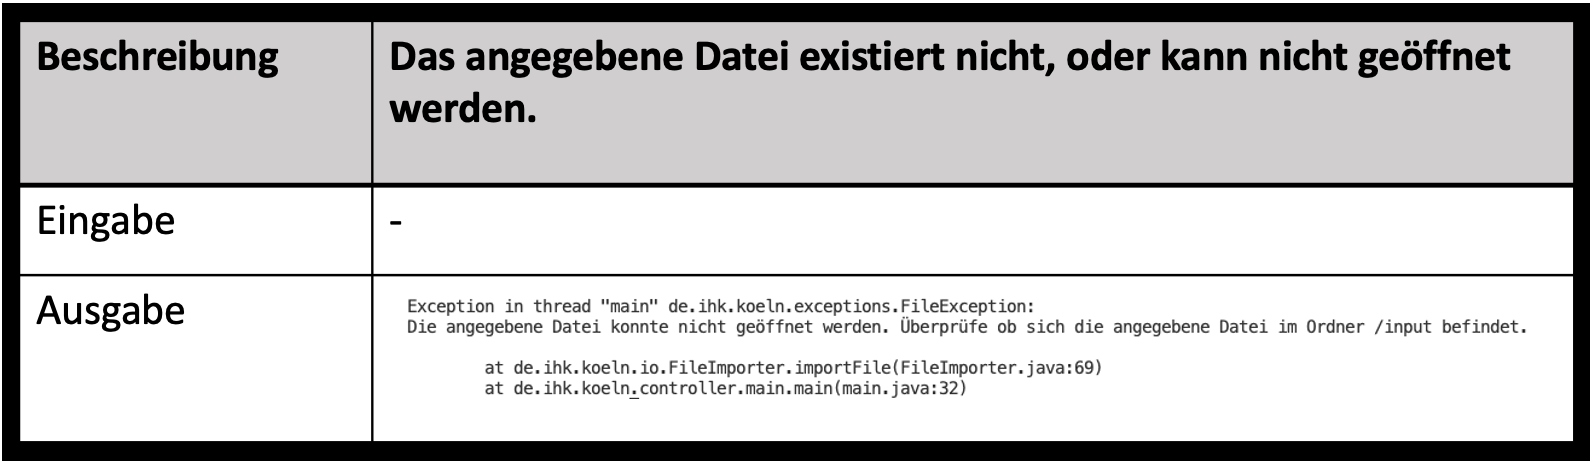
\includegraphics[width=\linewidth]{images/Tests/Fehlerfälle/FileException.png}
    \label{test:subsecpar:einlese-fehler}
\end{center}

\subsubsection{Datei besitzt keinen lesbaren Inhat}\label{test:subsec:kein-inhalt}
\begin{center}
    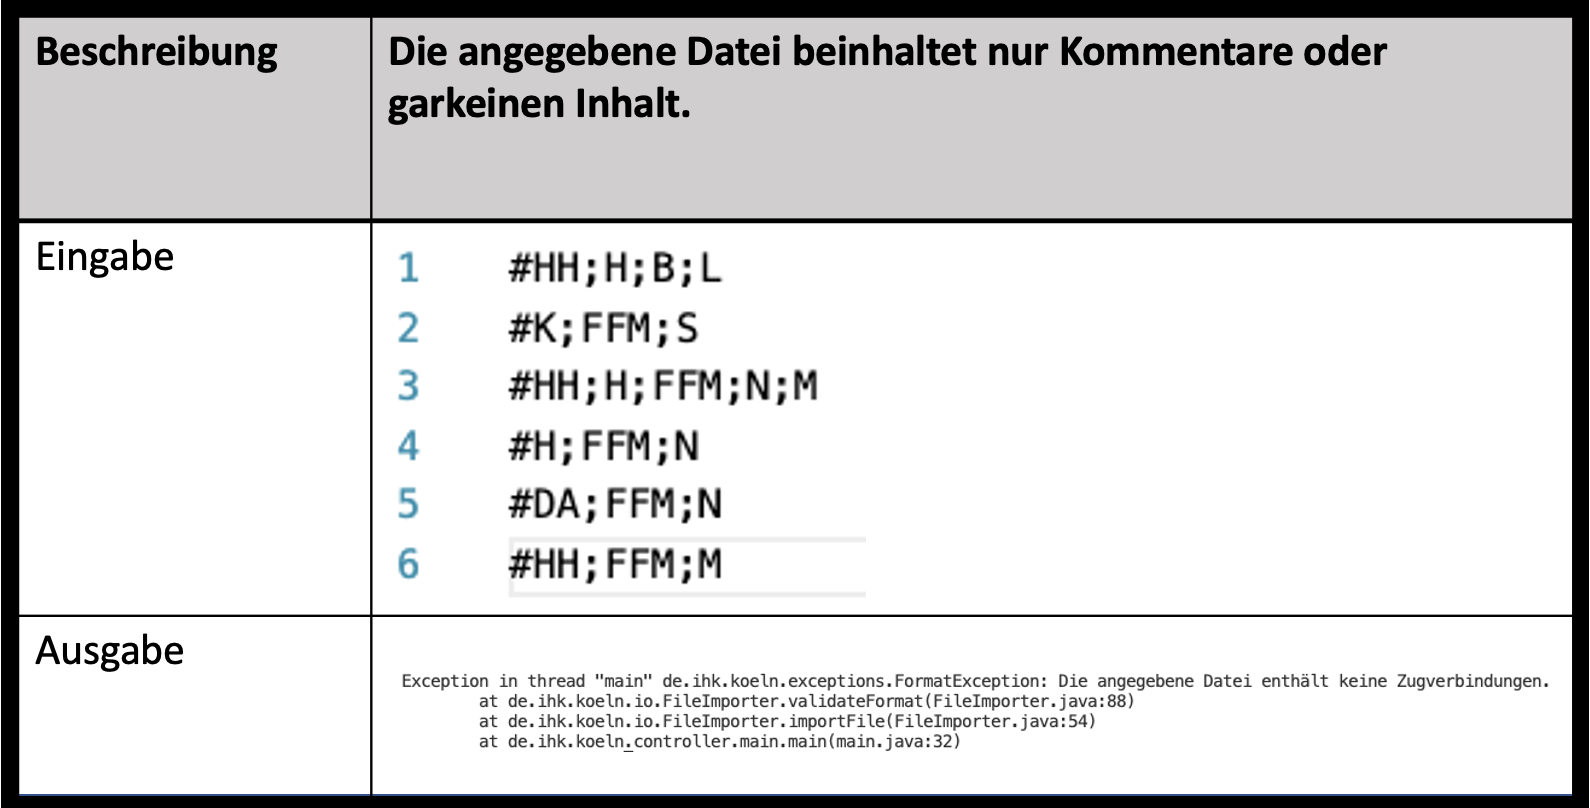
\includegraphics[width=\linewidth]{images/Tests/Fehlerfälle/LerreDatei.png}
    \label{test:subsecpar:leere-datei}
\end{center}

\subsubsection{Datei ist nicht im richtigen Format}\label{test:subsec:format}
\begin{center}
    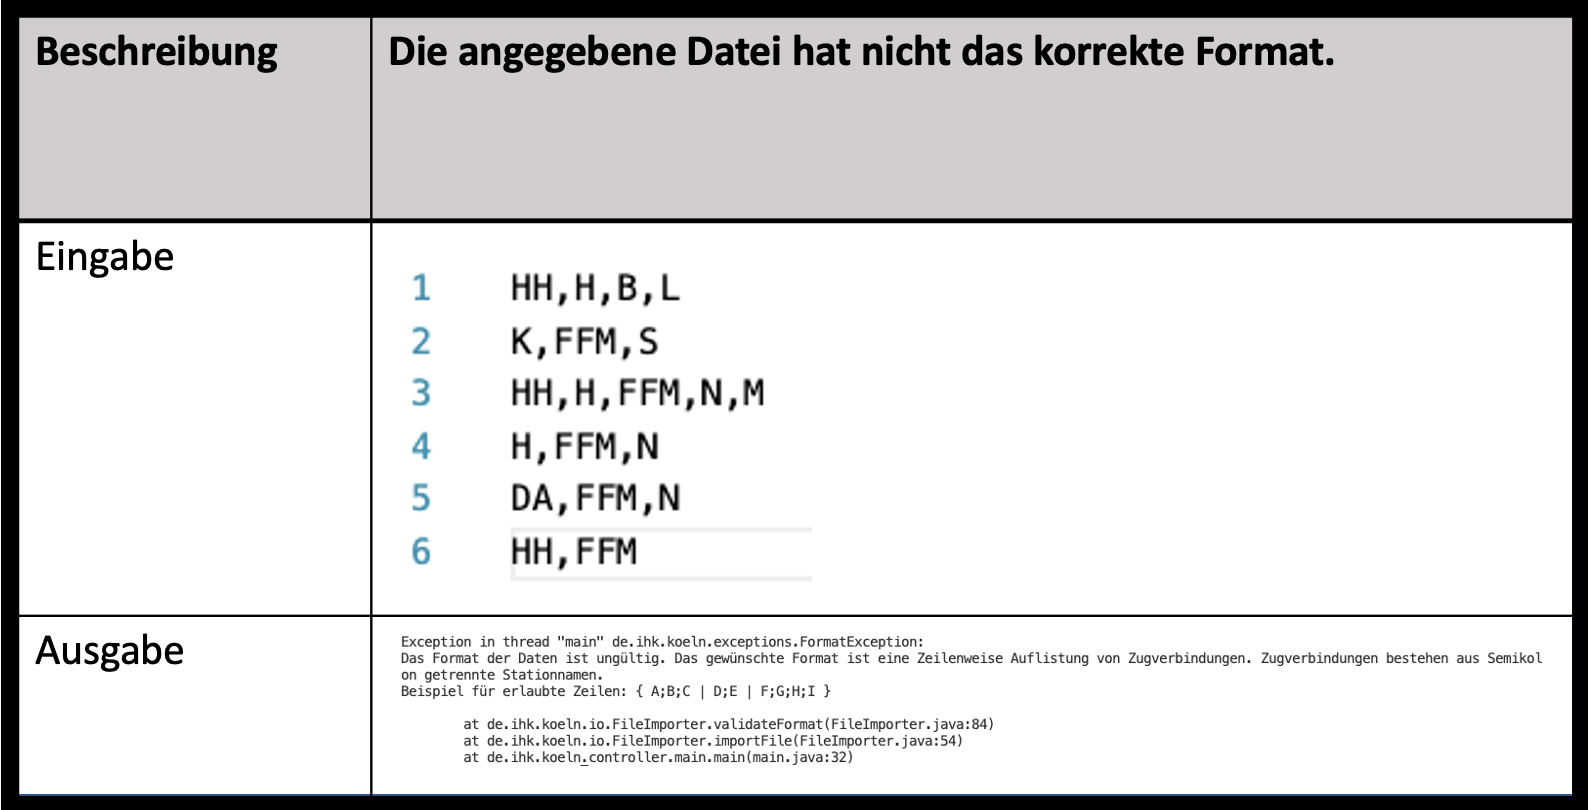
\includegraphics[width=\linewidth]{images/Tests/Fehlerfälle/FormatException.png}
    \label{test:subsecpar:format-fehler}
\end{center}

\subsubsection{Stationennamen sind nicht erlaubt}\label{test:subsec:namen-sind-nicht-erlaubt}
\begin{center}
    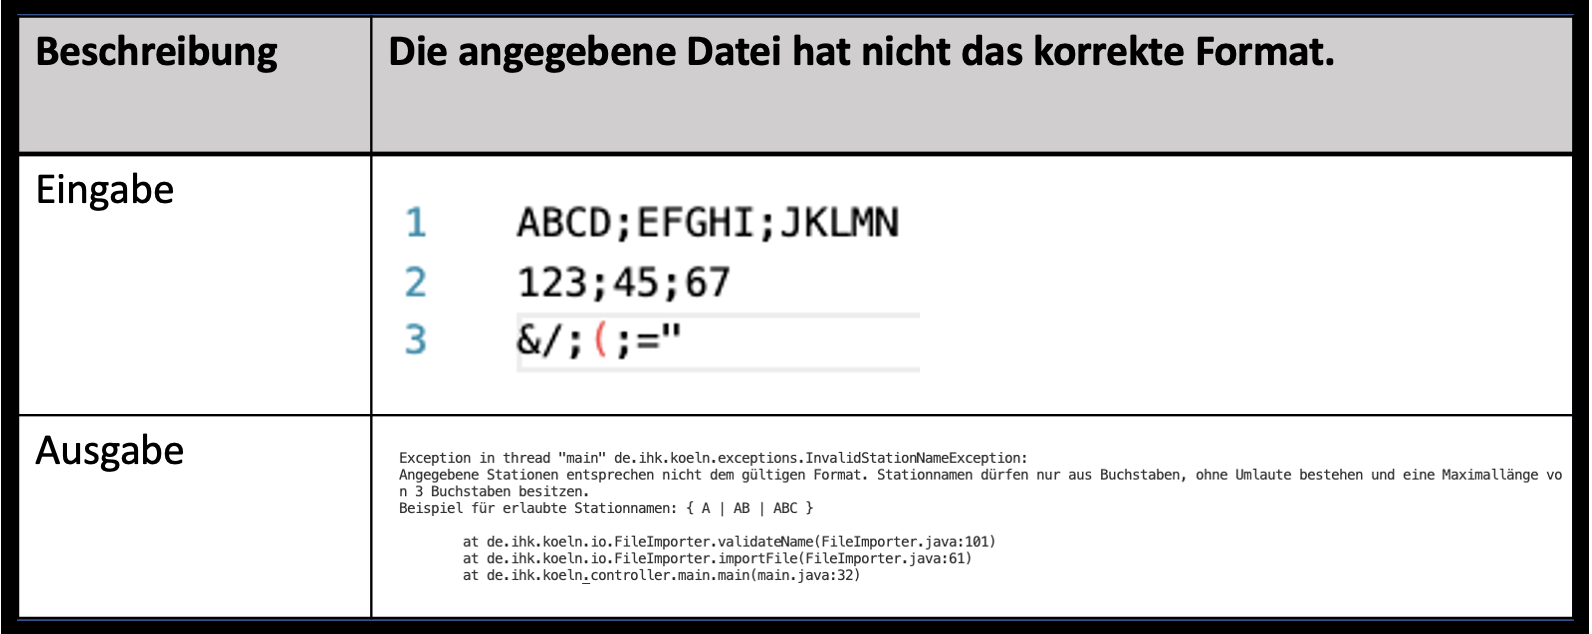
\includegraphics[width=\linewidth]{images/Tests/Fehlerfälle/InvalidNameException.png}
    \label{test:subsecpar:namen-sind-nicht-erlaubt}
\end{center}

\section{Grenzfälle}\label{test:sec:grenzfaelle}
\section{Sonderfälle}\label{test:sec:sonderfaelle}
